\chapter{Plan d'assurance qualité}

\section{Outils pour la gestion et la production des documents du projet}

    Les différents documents du projet seront produits à  l'aide de LaTeX et ensuite hébergés sur GitHub, un espace de travail collaboratif. Ce qui permettra à  chaque membre de l'équipe de suivre l'avancé des fichiers et de pouvoir les modifier à  distances.
    L'utilisation de l'outils Trello permettra également une bonne répartition des documents à produire entre les membres de l'équipe et d'informer les autres sur notre état d'avancement.

\subsection{Formalisme d'un document}

Pour chaque document, il faudra conserver dans un dossier sur GitHub :
\begin{itemize}
    \item le fichier au format texte.
    \item le make pour facilement créer le pdf.
    \item les différents fichiers insérés (images, tableaux, etc...).
\end{itemize}
On a choisi de ne pas garder le document pdf sur le dépôt pour une question d'espace mémoire.
\subsection{Procédure de création d'un document}

\begin{itemize}
    \item Créer le dossier qui va contenir les différents fichiers.
    \item Créer le fichier texte.
    \item Ecrire directement le titre (qui devra suivre une logique avec les autres fichiers texte).
    \item Les noms de fichiers seront du type : NomHexanome\_Titre.xxx
   \item Créer le Makefile.
\end{itemize}
Puis la rédaction du document pourra commencer.

\section{Mise en forme des fichiers}
\subsection{Les livrables en cours}

    Quelques règles devront être suivies pour permettre une bonne compréhension et relecture par tous les membres de l'équipe  :
\begin{itemize}
    \item Ne pas hésiter à  aérer le texte en passant à  la ligne, ou à  faire des listes.
    \item Séparer les idées en différents paragraphes.
    \item Penser à  l'indentation pour les nouveaux paragraphes.
\end{itemize}

\subsection{Les livrables finaux}
    Pour permettre une meilleure homogénéité entre tous les documents, la mise en forme finale des livrables se fera sous LaTeX. Une tête de page sera associée à  chaque page du livrable (sauf pour la page de garde) indiquant le titre de la section où on en est. Un pied de page sera associé à  chaque page du livrable pour indiquer le numéro de page.


\subsection{Page de garde}
Cette page devra contenir  :
\begin{itemize}
    \item le logo de l'INSA.
    \item les informations associées à l'INSA.
    \item le titre du projet.
    \item le titre du livrable.
    \item la période de réalisation du projet.
    \item l'image associées au projet.
    \item le nom de l'hexanôme.
    \item le nom des auteurs.
    \item le nom des enseignants.
\end{itemize}

\subsection{Sommaire}
    Le sommaire récapitulera l'ensemble des parties et sous parties du livrable. Elles seront indiquées par le titre de la partie (ou sous partie), et seront indiquées en lettres capitales pour les principales parties puis numérotées en chiffres arabes pour les sous parties. Chaque niveau de numérotation sera séparé par un point (Exemple : A.1.2). Le numéro de la page où se trouve la partie se situera à  droite. Des liens hypertextes dans le sommaire permettront d'aller directement à  la partie souhaitées.

\pagebreak
\section{Cycle de vie des livrables}

\begin{figure}[h]
    \centering
	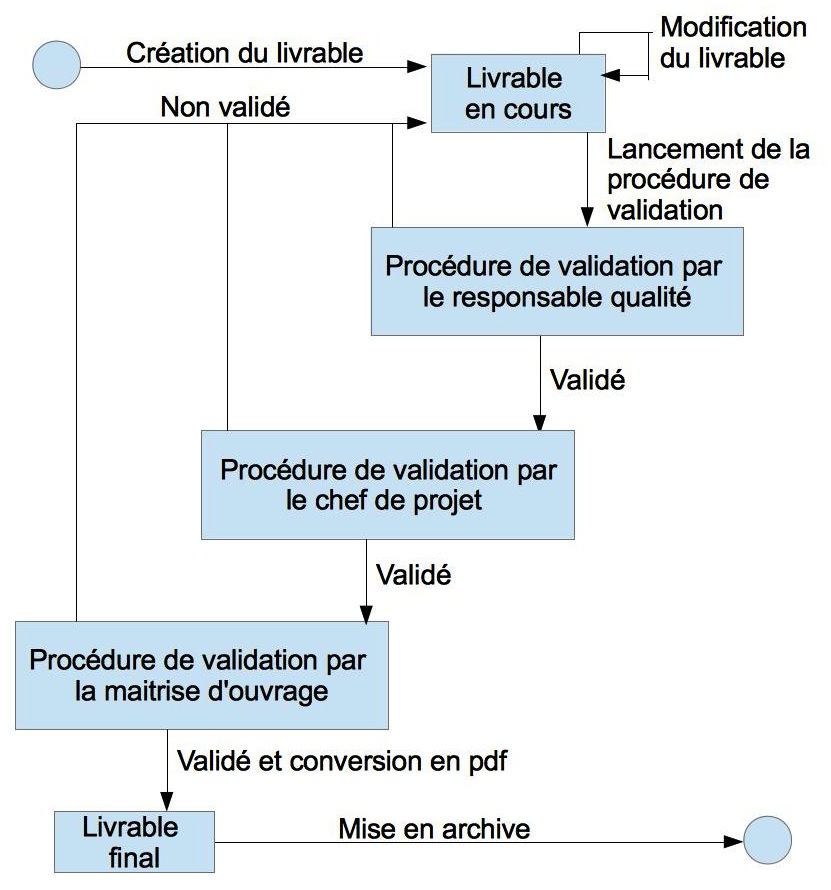
\includegraphics[width=140mm]{images/cycle_de_vie_des_docs.jpg}
    \caption{Cycle de vie des docs}
\end{figure}

\section{Procédure de validation interne}
  Une fois que l'auteur d'un livrable juge son travail fini, il contactera le responsable qualité qui fera alors une première relecture. Après validation une deuxième relecture sera faite par le chef de projet.
Si des modifications sont nécessaires, il y a deux solutions possibles  :
\begin{itemize}
    \item les modifications simples (fautes d'orthographes, présentations...) seront directement faites par le lecteur.
    \item les modifications plus importantes (gros irrespect du modèle de présentation, problème dans le contenu de fond...) entraineront une non validation et un retour à  l'auteur pour correction.
\end{itemize}
    L'auteur du livrable doit prévoir les temps de relectures et de corrections dans son planning pour pouvoir rendre son travail final en temps voulu.
    Le livrable passe donc par différents états  :
\begin{itemize}
    \item Version initiale  : c'est la première écriture du livrable, non relu par le chef de projet et le responsable qualité.
    \item Version modifiée  : livrable modifié depuis la dernière relecture mais non relu et validé par le chef de projet et le responsable qualité.
    \item Version validée  : livrable validé par le responsable qualité et le chef de projet. Doit être passer en pdf.
    \item Livrable final  : le fichier lu, approuvé et passé en pdf.
\end{itemize}

\section{Procédure de validation et de recette avec le client}
    A la date limite de rendu du livrable, l'équipe devra prendre contact avec le client pour débuter la procédure de validation (sauf indication de retard). Cela commencera par le dépôt du dit livrable sur la plateforme moodle dans la rubrique indiquée par le client.

    Si le document est irrécupérable (pour cause de document corrompu, introuvable...), le client pourra prendre contact avec le responsable communication de l'équipe pour demander un nouveau dépôt du livrable. La solution de livrer les documents par mail sera utilisée dans le cas où moodle deviendrait inutilisable.

    En cas de non validation par le client, ce dernier pourra contacter le responsable communication de l'équipe pour faire remonter les remarques aux membres du projet. En cas de non compréhension des propositions, le responsable communication entreprendra un échange de mail, ou une rencontre avec le client pour identifier clairement les modifications à  apporter.
    Une fois les corrections faites, un nouveau livrable sera déposé sur moodle, et le client informé par mail.

\section{Les outils utilisés durant le projet}
    Les documents seront gérés et partagés grâce à  GitHub. A chaque dépôt le membre de l'équipe devra écrire un commentaire indiquant les modifications apportées ou le but du document créé. Cela permettra un meilleur suivi des membres de l'équipe, et un retour facile à  une version antérieure en cas de problème.
    La rédaction initiale des livrables se fera sous n'importe quel éditeur de texte (selon la préférence de l'auteur). Mais la version finale avec sa mise en forme devra être faite sous LaTeX. LaTeX nous permettant une mise en forme plus rapide, et uniforme entre tous les documents.
Dans le but de suivre l'évolution du projet, le chef de projet utilisera Gantt Project pour les plannings, puis OpenOffice pour mettre à  jour des fiches tels que  :
\begin{itemize}
    \item Les fiches de suivi d'avancement des livrables (une par livrable)
    \item Les comptes rendus de réunion (une par réunion)
    \item Les tableaux de bord (une par réunion)
\end{itemize}

\pagebreak
\section{Les fiches}
\subsection{Tableau de bord}
\begin{figure}[h]
    \centering
    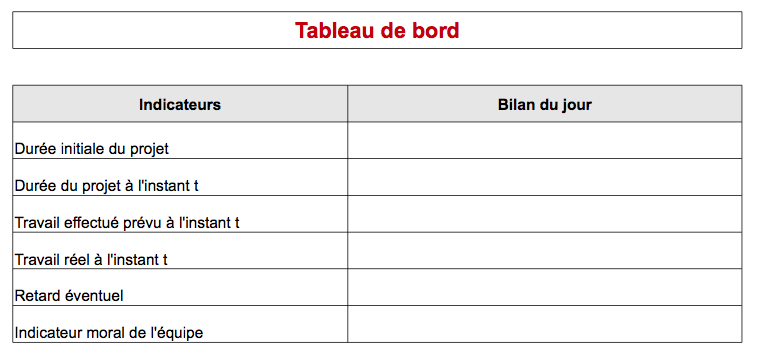
\includegraphics[width=140mm]{images/TblBord.png}
    \caption{Tableau de bord}
\end{figure}

\pagebreak
\subsection{Fiche de suivi d'avancement des livrables}
\begin{figure}[h]
    \centering
    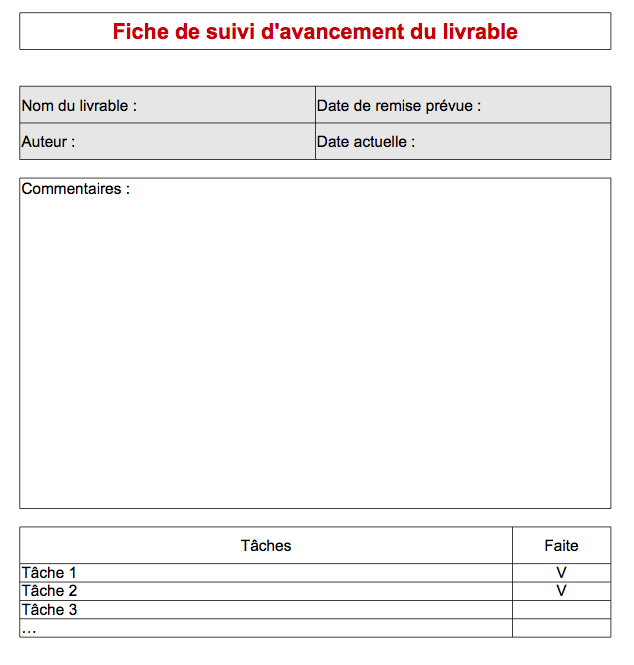
\includegraphics[width=140mm]{images/fiche_de_suivi_davancement_des_livrables.png}
    \caption{Fiche de suivi d'avancement des livrables}
\end{figure}

\pagebreak
\subsection{Journal de réunions}
\begin{figure}[h]
    \centering
    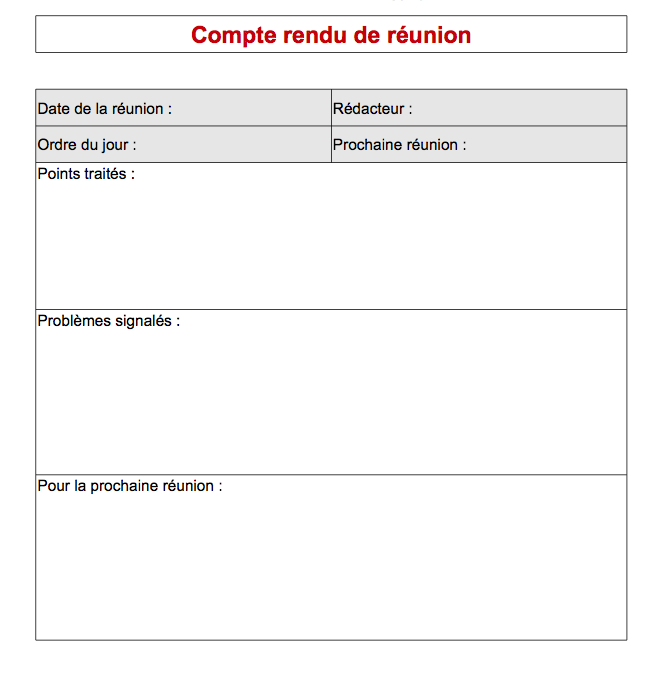
\includegraphics[width=140mm]{images/compte_rendu_reunion.png}
    \caption{Compte rendu réunion}
\end{figure}

\pagebreak
\begin{landscape}
\subsection{Fiche de suivi global}
\begin{figure}[h]
    \centering
    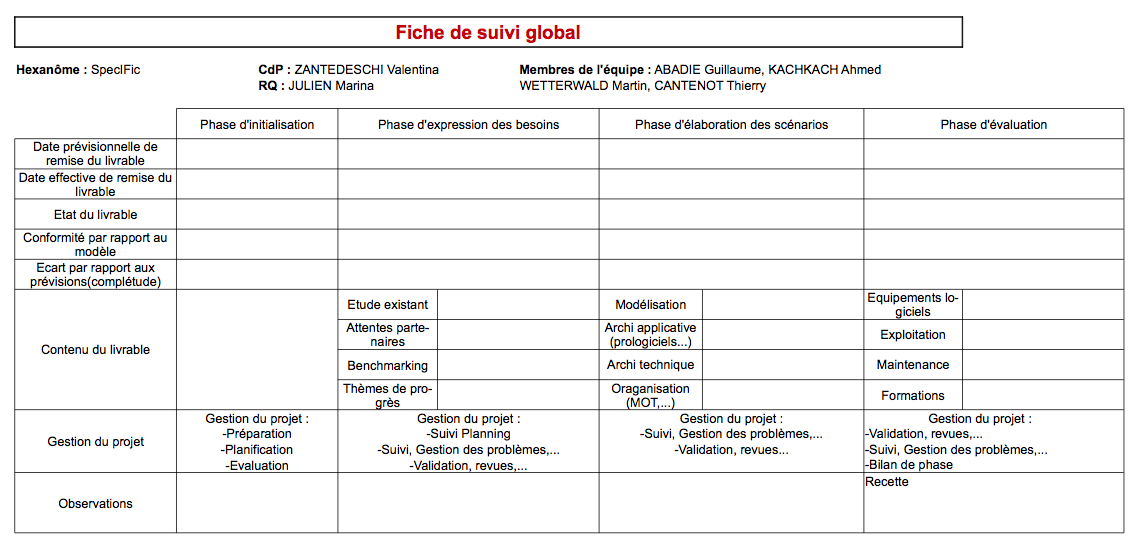
\includegraphics[width=220mm]{images/dashboard.png}
    \caption{Tableau de bord}
\end{figure}
\end{landscape}
